%% ═══════════════════════════════════════════════════════════════════════════
\subsection{Introduction}
\label{sec:res_intro}
%% ═══════════════════════════════════════════════════════════════════════════

Two claims are worth separating before any figure is given, because conflating them is the
easiest way to misread what follows. That the gap between declared and computed urgency
carries information about which supplier will fail is supported by the campaign. That the gap
can be converted into a well-calibrated probability attached to a named week is not, yet. The
distance between those two statements is the subject of
Sections~\ref{sec:res_armA_scored} and~\ref{sec:res_repair}, and the sample that bounds both
is stated wherever a figure is given.

Every number below is regenerated from raw artefacts by the derivation script described in
Section~\ref{sec:methods_repro}.

%% ═══════════════════════════════════════════════════════════════════════════
\subsection{The Delivered System}
\label{sec:res_system}
%% ═══════════════════════════════════════════════════════════════════════════

SupplyScore is delivered as a standalone Python application: 73 modules across 10 packages,
covered by 1\,831 automated test functions in 106 test files, driving a multi-page Dash web
interface over a multi-tenant SQLite persistence layer. The suite expands to 2\,044 collected
cases, of which 2\,028 pass and 15 are skipped for want of an optional dependency; one fails
on two missing image files referenced by a presentation script outside the library. All of the mathematical objects of
Section~\ref{sec:math_framework} are implemented and exercised: the six-block noisy-OR
aggregation, the AHP elicitation with its consistency gate, the Fuzzy BWM weighting, the
bidirectional DAG propagation, the asymmetric adequacy score, the Monte Carlo lead-time
estimate, the PROMETHEE~II network outranking and the systematic shock-simulation
criticality index.

Three operational capabilities carry what follows. The per-node explainability page
reconstructs any score term by term, which is what allowed the diagnosis in
Section~\ref{sec:res_mechanism} to be made from the application rather than by hand. The Excel
export produces frozen data for analysis outside the tool. And the hardened persistence layer
is what makes a campaign database an auditable record weeks after the run. Two pages carry
most of the operator's interaction with the system: the weekly review
(Figure~\ref{fig:hebdo}) and the criticality ranking (Figure~\ref{fig:criticite}).

\begin{figure}[htbp]
    \centering
    \includegraphics[width=\linewidth]{Images/4.Operations/weekly_review_annotated.png}
    \caption[The weekly review page]{The weekly review page, with its interface terms keyed
    into English. The four panels commit as one signed transaction.}
    \label{fig:hebdo}
\end{figure}

\begin{figure}[htbp]
    \centering
    \includegraphics[width=\linewidth]{Images/4.Operations/criticality_annotated.png}
    \caption[Network criticality ranking]{The criticality ranking a coordinator would use to
    decide where to look first: for each active node, the rise in the final customer's real
    urgency were that node to fail completely.}
    \label{fig:criticite}
\end{figure}

%% ═══════════════════════════════════════════════════════════════════════════
\subsection{Mechanical Validation: The Synthetic Dry Run}
\label{sec:res_dryrun}
%% ═══════════════════════════════════════════════════════════════════════════

Before any declaration data existed, the full campaign mechanics were exercised end to end on
a disposable database. Five iterations calibrated the scenario and eliminated engine
artefacts, and the final iteration replayed all nineteen turns with synthetic respondents
standing in for the eight declarants.

This is an engineering check, not a scientific one, and the reason is in how the synthetic
declarations were made: each is anchored on the node's own local real urgency, following
$1 + 8 \times U_{r,\text{local}}$ with a fixed panic, under-report or neutral bias per role. A
declaration built that way cannot lag the signal it is derived from, cannot under-report it
for long, and cannot react at all to a press event it never reads, so it returns not confirmed
or not applicable on all six hypotheses by construction.
Figure~\ref{fig:helios_dryrun_trajectories} shows that circularity: real urgency solid and
synthetic declared urgency dashed, tracking each other closely at every node rather than one
lagging or decoupling from the other.

What the run does establish is that injection, weekly decay, milestone drift, event
calibration, propagation, criticality, snapshotting and backup all run correctly under the
two-turns-per-day cadence the campaign requires. It also calibrated the null baseline
detector, a raw threshold $U_{r,\text{local}} \ge 0.5$, at precision $0.16$ and recall
$0.27$: the bar the adequacy signal must clear to demonstrate value beyond a raw KPI
reading.

\begin{figure}[htbp]
    \centering
    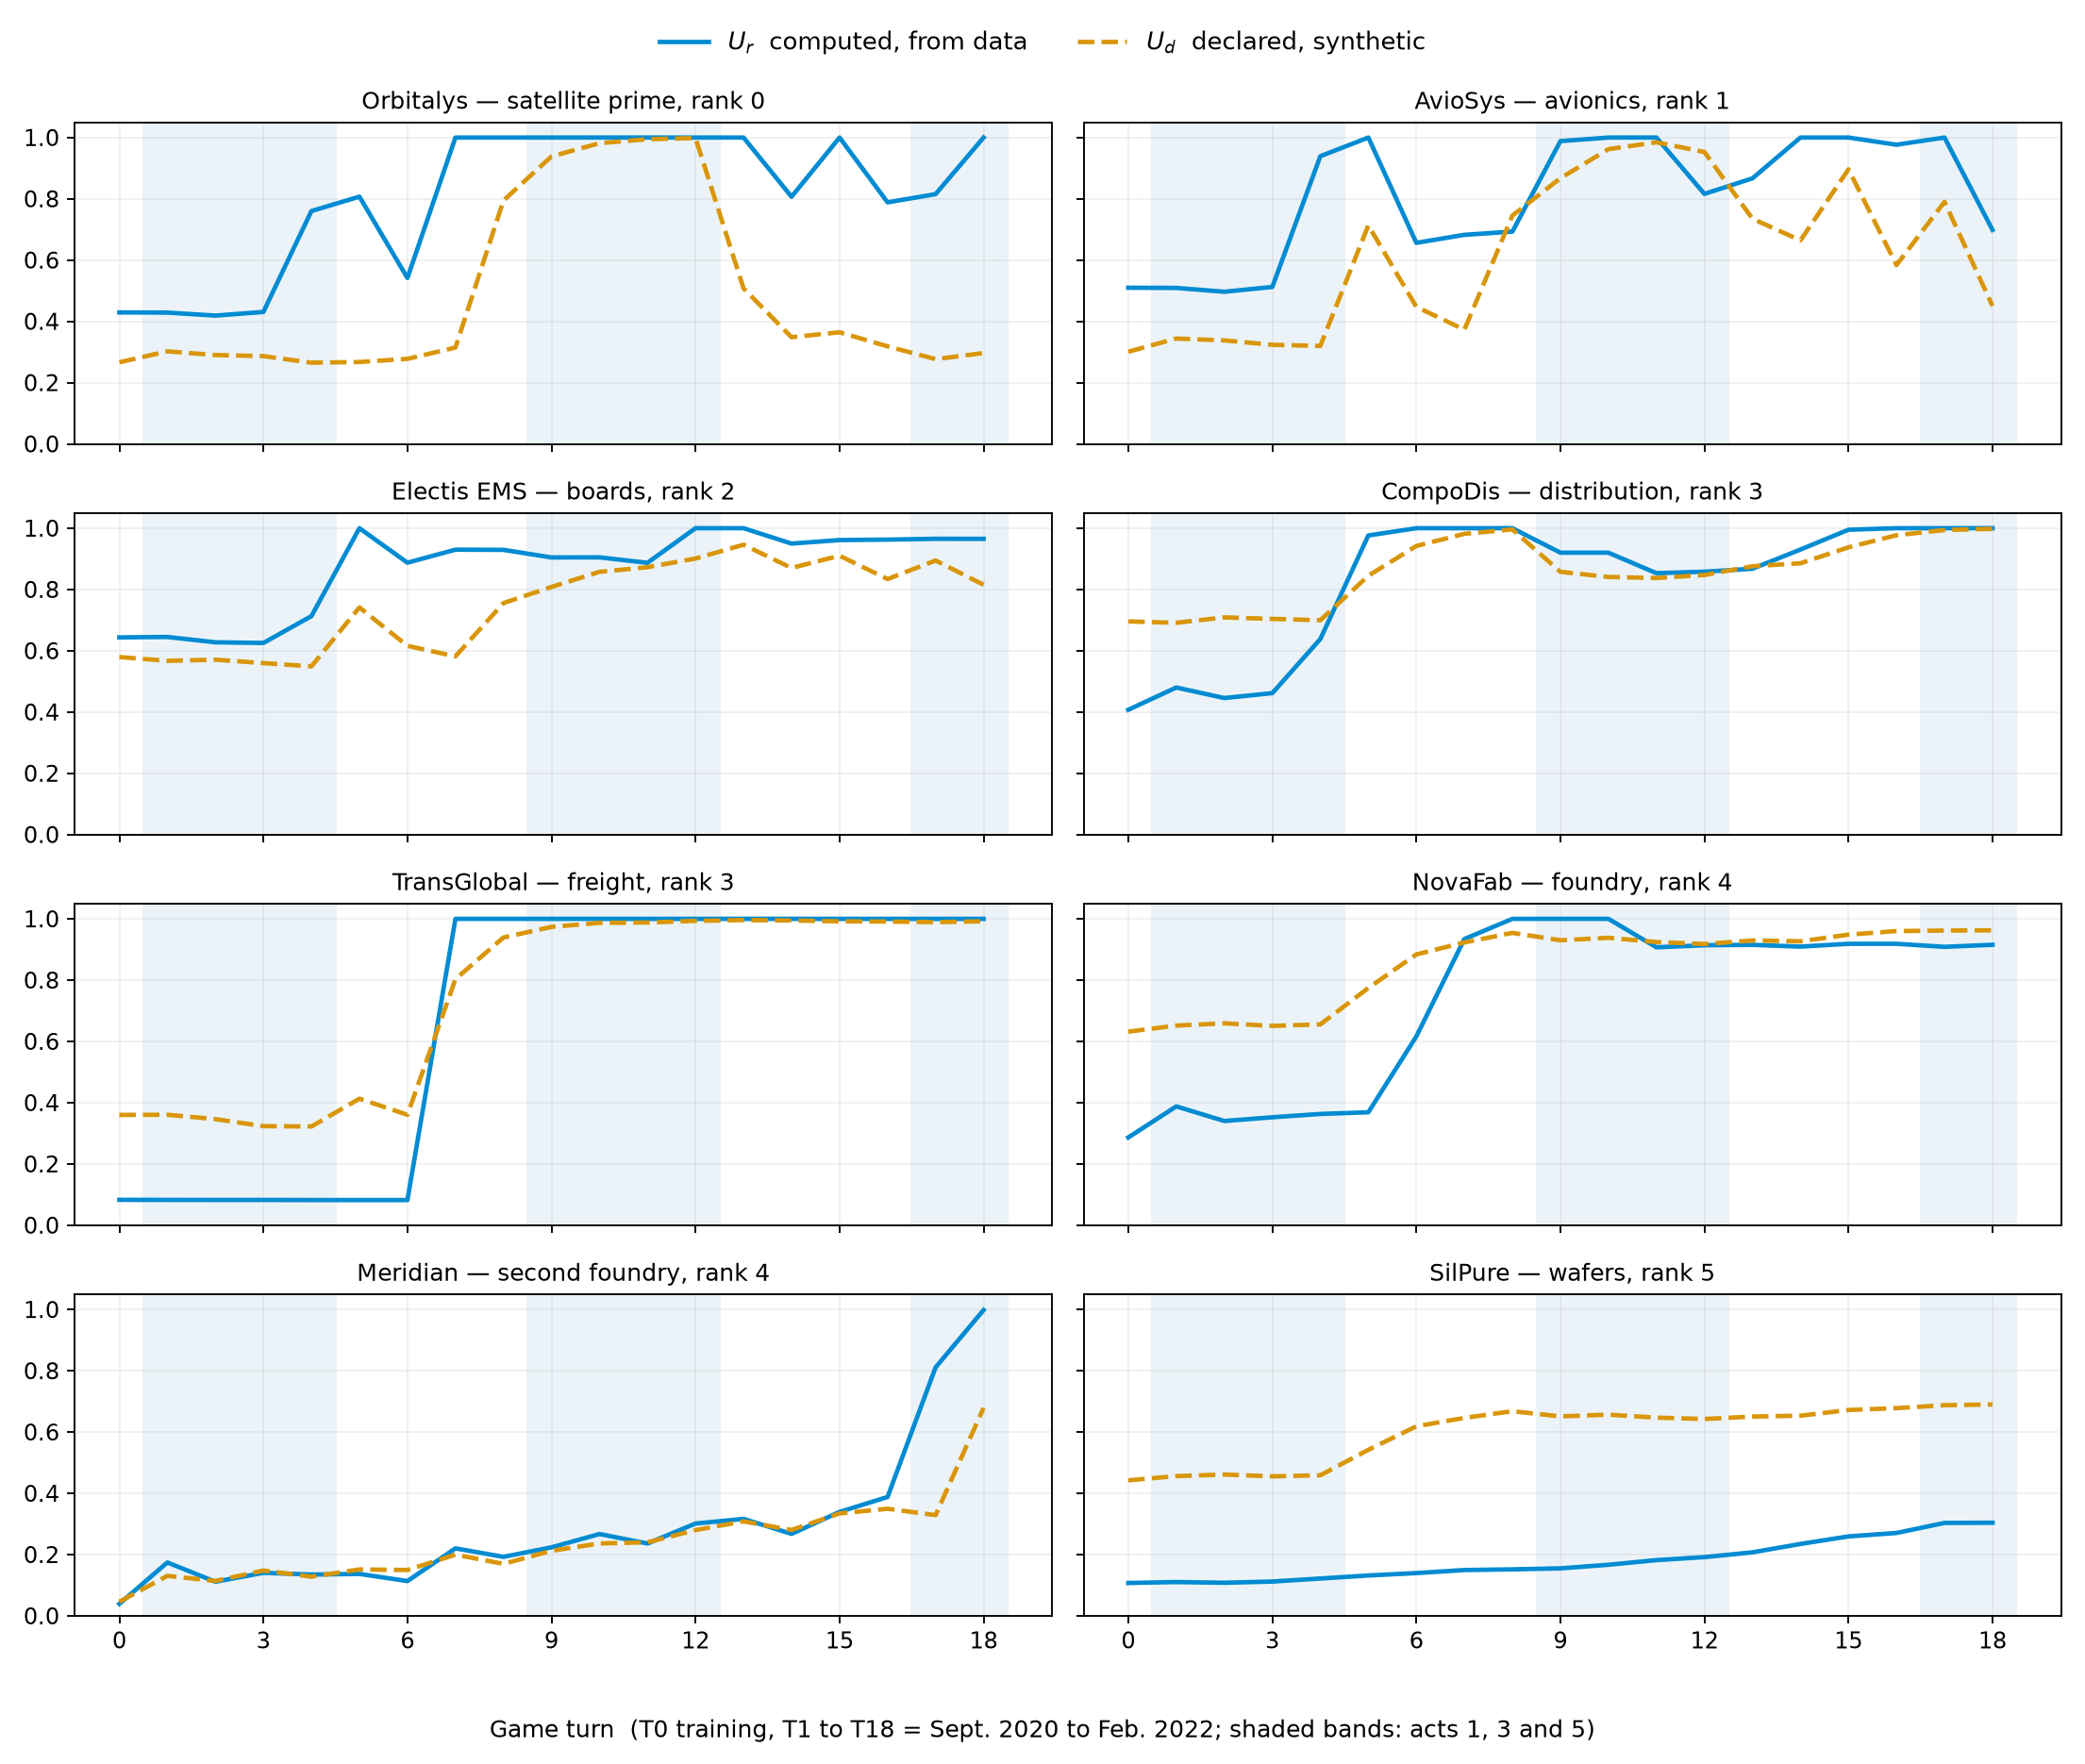
\includegraphics[width=\linewidth]{Images/helios_dryrun_trajectories_en.png}
    \caption{Real against synthetic declared urgency, dry run}
    \label{fig:helios_dryrun_trajectories}
\end{figure}

%% ═══════════════════════════════════════════════════════════════════════════
\subsection{Arm A: Blind Declaration by Eight Isolated Agents}
\label{sec:res_armA}
%% ═══════════════════════════════════════════════════════════════════════════

Arm A replaced the synthetic generator with the eight isolated agents of
Section~\ref{sec:methods_arms}. What matters here is that nothing was simulated around them:
each answered the real AHP questionnaire in character, pairwise comparisons and severity
scores passed through the production consistency-ratio code untouched, and campaign setup,
turn injection and submission went through the same weekly-cycle service a browser-based
participant would reach. Table~\ref{tab:helios_armA} gives the verdicts on the six
pre-registered tests.

\begin{table}[htbp]
\centering
\caption{Arm A verdicts on the six pre-registered hypotheses}
\label{tab:helios_armA}
\small
\begin{tabularx}{\linewidth}{>{\raggedright\arraybackslash}p{3.4cm} >{\raggedright\arraybackslash}p{2.4cm} X}
\toprule
\textbf{Test} & \textbf{Verdict} & \textbf{Measured value} \\
\midrule
H1 latency & Not confirmed & 3 of 8 nodes at lag $\ge 1$ turn (threshold: 5 of 8) \\
H2 early detection & Not confirmed & $H(\text{NovaFab})$ peaks at $0.017$ on turns 6 to 12
(threshold: $0.3$) \\
H3 criticality & Not confirmed & NovaFab top-1 on 7 of 10 informative turns, $70\%$
(threshold: $80\%$; saturated turns excluded per Section~\ref{sec:criticality}) \\
H4 predictive validity & Not confirmed & precision $0.00$, recall $0.00$ at $H \ge 0.5$ \\
H5 contagion & Confirmed & non-affected nodes: $\Delta U_d = +0.079$ on press turns against
$+0.005$ on calm turns \\
H6 hysteresis & Not applicable & real urgency shows no measurable decline over the recovery
turns \\
\bottomrule
\end{tabularx}
\end{table}

Two results stand out. H5 is confirmed: declared urgency at nodes that are not physically
affected rises by $0.079$ on press-event turns against $0.005$ on calm turns, matching the
pre-registered direction and ordering, which is the mere-urgency
effect~\autocite{zhu2018mere} reproduced at network scale. And H4 stays not confirmed for a
specific and informative reason: these agents read their briefing carefully and declared
urgency close to what it described, so $U_d$ tracks $U_r$ too closely to leave the gap that
$H$ is built to catch, more tightly even than the fixed-bias dry run, with
$H(\text{NovaFab})$ peaking at $0.017$ against $0.070$.

Read from the resulting project after the eighteenth turn, the network-average adequacy is
$65.5$, four of the eight nodes carry a hidden-risk reading above $0.1$, one carries a
false-urgency reading above $0.1$, and the worst-scoring node by a wide margin is Orbitalys at
$A = 15.3$ (Table~\ref{tab:armA_snapshot}).

Orbitalys' own explanation page traces the chain from a single scripted event to its score
without manual computation. Its next milestone had slipped past its deadline by turn 18,
which forces $u_{\text{time}}$ to $1$ under the rule of Table~\ref{tab:ur_blocks}; with the
node's real urgency already saturated by this cause alone, the page attributes the whole of
it to the local block and none to the upstream network. The agent playing Orbitalys declared
$U_d = 0.41$, so the hidden risk is $H = 0.59$, penalised through
Equation~\ref{eq:penalty} at $2.25 \times 0.59^{0.88} = 1.42$, giving
$A = 100 \times (e^{-1.42}-e^{-2.25})/(1-e^{-2.25}) = 15.3$, the same number the dashboard
reports. The network-wide PROMETHEE~II ranking places NovaFab and Orbitalys at the top of
the priority list, at $\phi = +0.220$ and $+0.215$, which are the expected bottleneck and
the node its own missed milestone makes most urgent. The same ranking carries a caveat the
tool raises on its own: on this run the time and performance blocks are perfectly
correlated, $\rho = 1.00$, which is exactly the composite-indicator risk flagged in
Section~\ref{sec:lit_mcdm}.

%% ═══════════════════════════════════════════════════════════════════════════
\subsection{What the Adequacy Signal Gets Right: Node-Level Targeting}
\label{sec:res_targeting}
%% ═══════════════════════════════════════════════════════════════════════════

The scoring that follows in Section~\ref{sec:res_armA_scored} asks whether the forecast layer
attaches correct probabilities to node-weeks. That is the right question for a forecast and
the wrong question for the instrument. A coordinator does not act on the proposition that node
$X$ has a $0.14$ chance of an adverse outcome between weeks $t+1$ and $t+4$; they act on a
shortlist of suppliers to look at this week. This subsection scores that, because it is the
decision the adequacy signal was designed to support, and because the answer differs from the
one below.

At each turn the eight nodes are ranked by hidden risk $H = [U_r - U_d]_+$, and the set
flagged at $H > 0.10$ is compared with the set of nodes that go on to miss at least one
milestone at its originally committed deadline, the definition of
Section~\ref{sec:res_target_trap}. Four of the eight nodes are positive under that definition:
the satellite prime, the avionics integrator, the electronics manufacturer and the foundry.
The comparison is at node level and prospective, since the flag at turn $t$ is confronted
with misses occurring later in the campaign. Nothing in it uses the forecast layer.

Table~\ref{tab:targeting} gives the two regimes the campaign separates, and the boundary
between them is the turn on which the scenario's foundry freeze becomes public.

\begin{table}[htbp]
\centering
\caption{Nodes flagged by hidden risk against nodes that later miss a commitment, arm A}
\label{tab:targeting}
\small
\begin{tabularx}{\linewidth}{l >{\centering\arraybackslash}X >{\centering\arraybackslash}X >{\centering\arraybackslash}X >{\centering\arraybackslash}X}
\toprule
\textbf{Regime} & \textbf{Turns} & \textbf{Precision} & \textbf{Recall} &
\textbf{False alarms per turn} \\
\midrule
Before the crisis is public & T0 to T5 & 1.00 & 0.75 & 0 \\
After & T6 to T18 & $\le 0.50$ & 0.25 & 1 to 3 \\
\bottomrule
\end{tabularx}
\end{table}

For six consecutive turns the signal flags exactly three nodes, all three of which later miss
a commitment, with no false alarm on any of the six. The fourth positive node is never
flagged early, so recall stops at three of four. On every one of those turns the worst-scoring
node of the eight is the satellite prime, which misses its turn-8 delivery and delivers at
turn 14: the flag precedes the miss by eight turns, and it is raised while that node's own
manager is declaring an urgency of $0.001$.

That last clause is the construction working as specified rather than a coincidence. The
flag does not come from a pessimistic declaration; it comes from an optimistic declaration
standing against a computed state that is not. A system aggregating indicators alone would
have ranked that node on its indicators. A system collecting declarations alone would have
believed it. Only the difference between the two carries this information, which is the
proposition the thesis set out to test and the one the literature review of
Section~\ref{sec:lit_gaps} found unaddressed.

\subsubsection{Why the Signal Degrades, and What the Sample Supports}

From turn 6 the precision falls to $0.50$ and the recall to $0.25$, for a structural reason.
Once the shortage is public every declarant raises their urgency, $U_d$ converges towards
$U_r$, and a quantity defined as $[U_r - U_d]_+$ shrinks by construction: a perception-gap
measure cannot survive the disappearance of the perception gap. The consequence is a scope
statement rather than a limitation to be repaired. The instrument is an early-warning device
and not a crisis-management one, and its useful window is the interval in which acting is
still cheap. The repair of Section~\ref{sec:res_repair} sharpens the flag without altering
which nodes it selects: at turn 3 the satellite prime scores $26.6$ out of $100$ against
$46.0$ for the next worst node, and after repair the same turn gives $2.2$ against $44.6$,
so the ordering is identical and the separation widens by an order of magnitude.

The standing of the result is bounded and stated plainly. It rests on eight nodes, four of
them positive, over one scripted scenario. A precision of $1.00$ sustained over six turns on
three flagged nodes is an encouraging observation and not an estimated rate: its Wilson
interval runs from $0.44$ to $1.00$, which Section~\ref{sec:res_power} reads against the
interval of the second chain. What would settle it is
more chains rather than a different model.

\subsubsection{The Second Chain, and the Boundary It Draws}
\label{sec:res_second_chain}

A second chain was then built and run: AIRB, an airframer's supply base of fifteen nodes and
thirty arcs over five ranks, with no exogenous shock at any point and three structurally
central suppliers set to degrade endogenously. Its milestone truth is derived from the
indicator trajectory rather than scripted, so a supplier that slows down misses its milestone
because it slowed down. Fifteen declarants, one per node, each seeing only its own monthly
sheet and its own past declarations, played all nineteen turns.

On that chain the adequacy signal does not select the failing nodes at all: across all
nineteen turns, precision at rank three is $0.00$ for both $[U_r - U_d]_+$ and the adequacy
score, against a base rate of $0.20$, while the forecast layer scored on the same runs holds
at $0.56$.

The mechanism is legible in the snapshots and is not a failure of aggregation. The three
degrading suppliers declare the highest urgencies in the chain from turn~0 onwards, before
their indicators have moved: $U_d = 0.94$, $0.88$ and $0.98$ at turn~0, still $0.97$ and
$0.96$ at turn~16 against a computed $U_r$ of $1.00$. A quantity defined as $[U_r - U_d]_+$
is then bounded by $0.03$. Nothing is concealed, so nothing is detected. The nodes that top
the gap ranking at every turn are the downstream assemblers, whose local urgency is
\emph{zero} and whose computed $U_r$ is inherited entirely through the graph from suppliers
they cannot observe.

This is a boundary rather than a refutation, and it is sharper than the scope statement above.
The role cards of those three suppliers described concealers, and the declarants behaved as
such in prose, turn after turn, writing that they would put off calling their customers and
keep overtime in reserve. At the same turns they marked near-maximal severity on the
questionnaire. They minimised in \emph{action} and maximised in \emph{measurement}. The
questionnaire asks what an actor perceives; withholding is something an actor does. A gap
defined between a computed state and a declared perception therefore detects blindness, not
discretion. The synthetic declarants of the semiconductor campaign carried a bias applied to
the number itself, so the gap opened and precision reached $1.00$; a declarant that reasons
does not lower the number.

The claim that survives both chains is therefore narrower: the perception gap is informative
where declarants misjudge their own state, and silent where they judge it correctly and simply
do not escalate. Distinguishing those two failure modes requires an instrument that observes
escalation behaviour and not only declared severity, which the present design does not
provide. Section~\ref{sec:future_work} states it first rather than as a caveat, because it
bears on what the instrument measures and not merely on how well.

%% ═══════════════════════════════════════════════════════════════════════════
\subsection{Arm A Rescored: Discrimination Without Calibration}
\label{sec:res_armA_scored}
%% ═══════════════════════════════════════════════════════════════════════════

The hypothesis verdicts above test the adequacy signal at a single threshold, and a single
operating point cannot distinguish a forecast that orders outcomes badly from one that orders
them well but announces the wrong numbers. This subsection therefore scores all 120
prospective forecasts of arm A, covering turns 4 to 18 across eight nodes, against the
production outcome definition of Section~\ref{sec:methods_scoring}.
Table~\ref{tab:armA_scores} gives the results at each horizon.

\begin{table}[htbp]
\centering
\caption{The arm A forecast layer, scored by horizon}
\label{tab:armA_scores}
\small
\begin{tabularx}{\linewidth}{c >{\centering\arraybackslash}X >{\centering\arraybackslash}X >{\centering\arraybackslash}p{3.0cm} >{\centering\arraybackslash}X >{\centering\arraybackslash}X}
\toprule
\textbf{Horizon} & \textbf{Positives} & \textbf{Base rate} & \textbf{AUC [95\% CI]} &
\textbf{Brier} & \textbf{Brier skill} \\
\midrule
1 week  & 2 & 0.017 & 0.555 [0.470, 0.639] & 0.130 & $-6.93$ \\
2 weeks & 4 & 0.033 & 0.372 [0.258, 0.492] & 0.166 & $-4.14$ \\
3 weeks & 5 & 0.042 & 0.428 [0.315, 0.546] & 0.191 & $-3.77$ \\
4 weeks & 6 & 0.050 & 0.485 [0.389, 0.583] & 0.207 & $-3.36$ \\
\bottomrule
\end{tabularx}
\end{table}

There is no discrimination to speak of. The AUC ranges from $0.372$ to $0.555$ and every
95\% interval contains $0.5$, so on this campaign the forecast does not order node-weeks
better than chance. That statement carries its sample size: the positive class contains
between 2 and 6 observations depending on horizon, far too few to support a confident claim in
either direction, so the campaign provides no evidence of discrimination rather than refuting
it.

The calibration result is much stronger, because it does not depend on the small positive
class in the same way. The Brier skill against climatology is between $-3.36$ and $-6.93$,
meaning the forecast is between four and eight times worse, in mean squared error, than a
trivial forecaster that announces the base rate every time.
Figure~\ref{fig:armA_reliability} bands the four-week forecasts by announced probability and
compares the mean announced value with the observed frequency in each band.

The pattern is unambiguous, each marker's area proportional to the number of forecasts in
its band. Where the model announces a low
probability it is right: 74 forecasts announcing a mean of $0.070$ were followed by an adverse
outcome $8.1\%$ of the time. Where it announces a high probability it is wrong every single
time: twenty-one forecasts announced a mean of $0.948$ and none was followed by the outcome it
predicted. The confusion matrix at the threshold of $0.5$ records 0 true positives, 21 false
positives, 6 false negatives and 93 true negatives.

Hypothesis H4 is stated on a different quantity and should not be read off that matrix: it
tests the hidden risk $H$, not the four-week forecast, at its own threshold of $H \ge 0.5$.
Measured on the campaign database through the production calibration service, that second
matrix reads 0 true positives, 3 false positives, 8 false negatives and 141 true negatives
over 152 node-weeks at four weeks. The two signals fail at the same threshold and for related
reasons, and both return precision and recall of exactly zero, but they are separate
measurements and the H4 verdict rests on the second.

\begin{figure}[htbp]
    \centering
    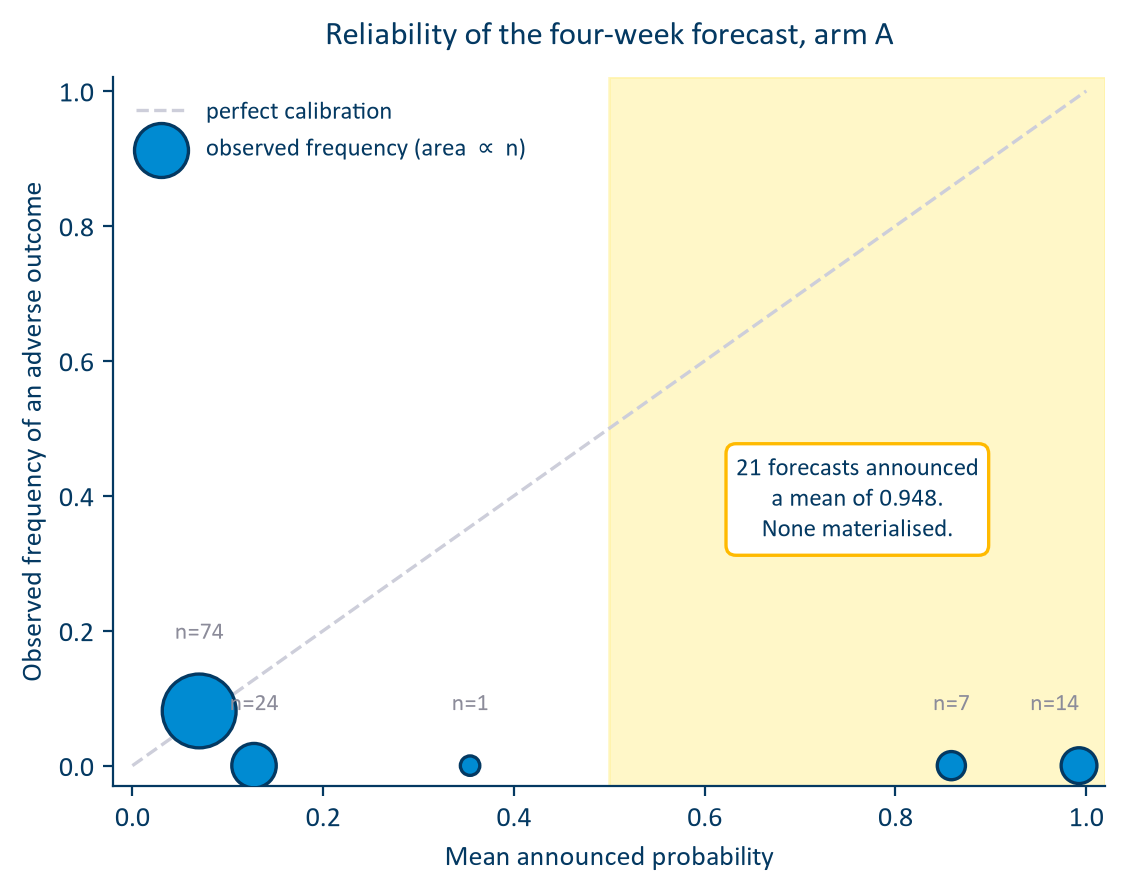
\includegraphics[width=0.86\linewidth]{Images/armA_reliability.png}
    \caption{Reliability of the four-week forecast, arm A}
    \label{fig:armA_reliability}
\end{figure}

The two failures are therefore of different kinds, and this is the dissociation that
Murphy's decomposition anticipates~\autocite{murphy1973vector}: the ordering is
uninformative, and the level is badly wrong at the top of the range while being close to
right at the bottom.

An obvious objection is right-censoring: forecasts made near the end of the campaign have
observation windows extending past the last turn, so if the confident ones were concentrated
there, censoring rather than miscalibration would explain the result. They are not. The
twenty-one confident forecasts are spread over turns 5 to 18 and across seven of the eight
nodes, and repeating the scoring with every forecast whose window runs past the final turn
removed leaves $n = 88$, still 0 true positives against 16 false positives, with the Brier
skill moving from $-3.36$ to $-7.82$: worse rather than better.

\subsubsection{The Mechanism}
\label{sec:res_mechanism}

Figure~\ref{fig:utime_defect} states the defect before the evidence for it.

\begin{figure}[htbp]
\centering
\begin{tikzpicture}[x=1cm, y=1cm, font=\scriptsize,
    st/.style = {bloc, text width=2.6cm, minimum height=0.85cm},
    dead/.style = {blocAlerte, text width=2.6cm, minimum height=0.85cm}]

\node[st] (ev)   at (1.7, 1.2) {a critical event\\is declared};
\node[st] (kpi)  at (5.3, 1.2) {the risk block\\rises};
\node[dead] (lt) at (8.9, 1.2) {the lead-time\\parameters};
\node[st] (ut)   at (12.5, 1.2) {$u_{\text{time}}$, and the\\milestone forecast};

\draw[fleche] (ev) -- (kpi);
\draw[fleche] (kpi) -- (lt);
\draw[flecheCoupee, draw=altenOchreDark, line width=1.3pt] (lt) -- (ut);
\node[etiquette, anchor=south, text=altenOchreDark] at (10.7, 1.75) {never arrives};

\draw[fleche] (ev.south) -- (1.7, 0.1) -- (12.5, 0.1) -- (ut.south);
\node[etiquette, anchor=north, fill=white] at (7.1, 0.1)
     {the only channel that does reach the forecast is the calendar};

\node[etiquette, anchor=north, text width=11cm] at (7.1, -0.55)
     {consequence: the four-week probability and the milestone-miss probability never differ
      by more than $0.020$ across the twenty-one confident forecasts, because nothing but the
      milestone channel contributes to either};

\end{tikzpicture}
\caption[Where the time block stops listening]{The defect located in this section. An event
raises the risk block but never reaches the lead-time parameters that feed
$u_{\text{time}}$, so the milestone forecast is driven by the calendar alone and is blind to
the shocks the scenario injects.}
\label{fig:utime_defect}
\end{figure}

The confident tail has a single source, and the explainability layer of
Section~\ref{sec:explain_export} makes it visible without instrumentation: across all
twenty-one confident forecasts, the four-week probability and the milestone-miss probability
never differ by more than $0.020$. Nothing but the milestone channel contributes to it.

Set against the registry, this is decisive. Of the eighteen milestones in the campaign, ten
completed and eight remained active, none was abandoned, and exactly one was still open past a
deadline that had fallen inside the campaign. The model announced near-certain misses for
AvioSys, CompoDis, \'Electis, NovaFab, TransGlobal and Meridian, and all of them delivered.
That reading is more forgiving than it appears, because the registry stores each milestone's
\emph{current} deadline and a replanning overwrites it, so a milestone re-dated and
subsequently delivered is recorded as completed. Read against the deadline each node
originally committed to, six of the eleven milestones whose original deadline fell inside the
campaign were missed, and five of the twenty-one confident forecasts were followed by a missed
original commitment within four weeks rather than none. The confident tail remains wrong far
more often than right, but the distance between zero of twenty-one and five of twenty-one is
produced entirely by which deadline the truth is read against, which is the subject of
Section~\ref{sec:res_target_trap}.

The same defect is visible directly in the state snapshots, from the opposite side. Reading
the $u_{\text{time}}$ block at turn 6, the turn on which the scenario's one critical event
lands, gives the values of Table~\ref{tab:u_time_turn6}.

Six of the eight nodes read as numerically zero in the middle of a crisis and the seventh
reads as saturated: the block behaves as a step function rather than a risk gradient, either
off or fully on. The cause is structural. The block compares a lead-time distribution against
the time remaining to the next deadline, while the scripted events act on capacity, cost and
failure probability without touching any quantity on the time axis, so a shock never moves
what the milestone probability is computed from. The strongest form of the evidence depends on
no scoring choice at all: across the whole campaign, eight nodes and 41 indicator snapshots
each, the accumulated-delay field the block would need was written a non-zero value exactly
zero times.

This is a defect in the model rather than a property of the scenario, and it is the one
finding of the campaign with a concrete repair. It also invalidates, for this run, the assumption of
Section~\ref{sec:model_blocks} that each block contributes useful information to the
aggregate. One block did not.

%% ═══════════════════════════════════════════════════════════════════════════
\subsection{The Target-Definition Trap}
\label{sec:res_target_trap}
%% ═══════════════════════════════════════════════════════════════════════════

The scores above depend on a choice that is easy to overlook: what counts as an adverse
outcome. Section~\ref{sec:methods_scoring} uses the production definition, requiring a missed
milestone, an abandoned node or an event of gravity critical or defect. Two alternatives are
worth scoring the identical forecasts against: the one an evaluator without access to the
model's own definition would reach for, any event recorded on the node; and one that keeps the
production definition intact but reads a missed milestone against the deadline the node
originally committed to, dropping the forecasts whose window runs past the last campaign turn.
Table~\ref{tab:target_trap} gives the three.

\begin{table}[htbp]
\centering
\caption{The same forecasts under three outcome definitions}
\label{tab:target_trap}
\small
\begin{tabularx}{\linewidth}{X >{\centering\arraybackslash}p{1.1cm}
                                 >{\centering\arraybackslash}p{1.7cm}
                                 >{\centering\arraybackslash}p{1.3cm}
                                 >{\centering\arraybackslash}p{1.9cm}}
\toprule
\textbf{Outcome definition (4-week horizon)} & \textbf{$n$} & \textbf{Base rate} &
\textbf{AUC} & \textbf{Brier skill} \\
\midrule
Production definition: missed milestone, abandonment, or critical event & 120 & 0.050 &
0.485 & $-3.36$ \\[3pt]
Naive definition: any recorded event & 75 & 0.387 & 0.484 & $-0.64$ \\[3pt]
Original-commitment definition: production outcome, deadline as first committed, censored
points excluded & 90 & 0.289 & 0.654 & $-0.55$ \\
\bottomrule
\end{tabularx}
\end{table}

The model is identical, the forecasts are identical, and the horizon is identical. Only the
definition of truth changes. Between the first two rows the measured base rate moves from
$5.0\%$ to $38.7\%$ and the Brier skill improves by a factor of more than five, from $-3.36$
to $-0.64$. An analyst choosing the easier target would report a system that appears five
times better calibrated without a single line of the model having changed.

The third row moves the answer in a different direction and for a defensible reason rather
than a convenient one. Holding the definition of an adverse outcome fixed and only changing
which deadline a milestone is judged against carries the Brier skill from $-3.36$ to $-0.55$
and the AUC from $0.485$, indistinguishable from chance, to $0.654$. The argument for
preferring it is about what a forecast is for rather than about statistics: a replanning is
itself the formal admission of a slip, so a truth in which re-dating erases the miss scores
the forecast against an outcome it was built to warn about before the re-dating happened. It
is the definition used for the re-measurement of Section~\ref{sec:res_repair}, and stating
which of the three any figure refers to is not pedantry: the three disagree by more than any
modelling decision taken in this work.

\begin{figure}[htbp]
    \centering
    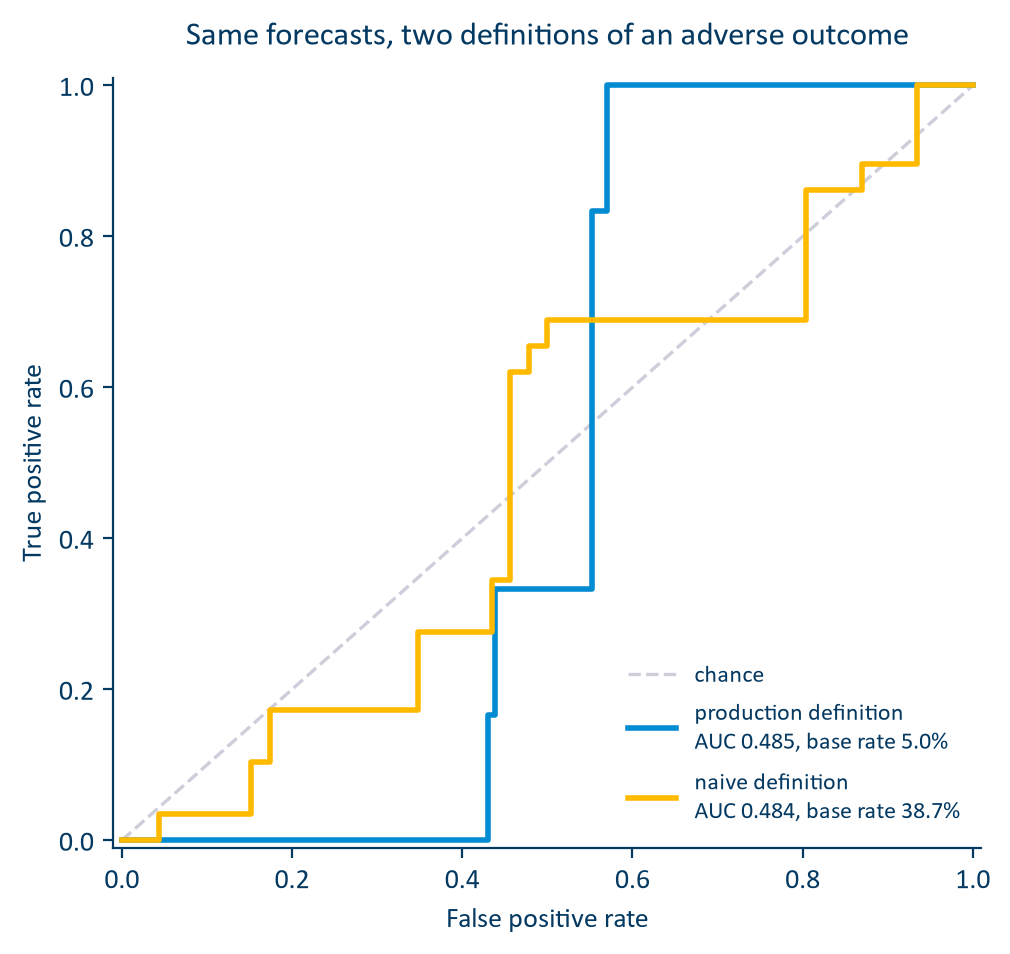
\includegraphics[width=0.86\linewidth]{Images/armA_roc.png}
    \caption{ROC under both outcome definitions}
    \label{fig:armA_roc}
\end{figure}

Discrimination, by contrast, is almost untouched, moving from $0.485$ to $0.484$
(Figure~\ref{fig:armA_roc}). That contrast is itself informative: the ordering of node-weeks is
a property of the forecast, while the apparent quality of the probabilities is substantially a
property of how often the target fires, since a frequent target flatters a forecaster who
announces high probabilities. A calibration figure reported without its outcome definition is
therefore close to meaningless, and the definition belongs in the pre-registration alongside
the thresholds, where the H1 to H6 register does not currently carry it.

%% ═══════════════════════════════════════════════════════════════════════════
\subsection{How Much of This Is Signal}
\label{sec:res_power}
%% ═══════════════════════════════════════════════════════════════════════════

Every score reported so far is a point estimate resting on a positive class of between one
and six observations. The protocol of Section~\ref{sec:methods_scoring} fixed in advance how
such estimates are to be read; this section applies it to the headline claims and states what
survives. Nothing new is measured here. The forecasts, the labels and the scores are the ones
already reported, and only their uncertainty is added.

Table~\ref{tab:auc_tests} tests every arm~A discrimination figure against chance, and
Figure~\ref{fig:auc_forest} draws the same eight rows against the $0.5$ line.

\begin{table}[htbp]
\centering
\caption[Discrimination against chance]{Arm A discrimination against chance, under two
outcome definitions. The interval is the percentile bootstrap; the $p$-value is the exact
conditional test of $\mathrm{AUC}=0.5$}
\label{tab:auc_tests}
\small
\begin{tabularx}{\linewidth}{@{}X c c c c c@{}}
\toprule
\textbf{Outcome definition} & \textbf{$h$} & \textbf{$n$} & \textbf{pos.} &
\textbf{AUC [95\% boot.]} & \textbf{$p$} \\
\midrule
Production            & 1w & 120 & 2 & $0.555$ $[0.470, 0.639]$ & $0.797$ \\
                      & 2w & 120 & 4 & $0.372$ $[0.258, 0.492]$ & $0.388$ \\
                      & 3w & 120 & 5 & $0.428$ $[0.315, 0.546]$ & $0.590$ \\
                      & 4w & 120 & 6 & $0.485$ $[0.389, 0.583]$ & $0.904$ \\
\addlinespace
Naive, any event      & 1w &  75 & 11 & $0.603$ $[0.404, 0.786]$ & $0.279$ \\
                      & 2w &  75 & 19 & $0.601$ $[0.456, 0.741]$ & $0.192$ \\
                      & 3w &  75 & 25 & $0.545$ $[0.409, 0.675]$ & $0.529$ \\
                      & 4w &  75 & 29 & $0.484$ $[0.358, 0.621]$ & $0.823$ \\
\bottomrule
\end{tabularx}
\end{table}

\begin{figure}[htbp]
    \centering
    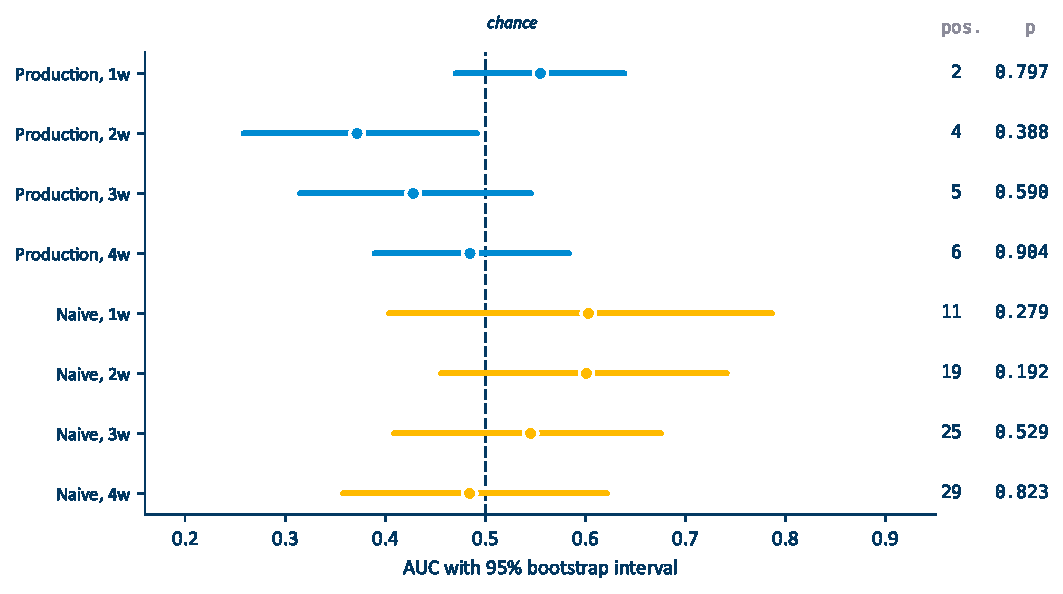
\includegraphics[width=0.94\linewidth]{Images/auc_forest.pdf}
    \caption[Discrimination against chance]{Every arm~A AUC with its bootstrap interval, read
    against the dashed chance line. An interval crossing that line is a result the campaign
    cannot separate from chance. The positive-class size and the exact $p$-value are given at
    the right of each row.}
    \label{fig:auc_forest}
\end{figure}

Not one of the eight is distinguishable from chance. The smallest $p$-value in the table is
$0.192$, and it belongs to the naive definition, the one this thesis argues against using.
The claim of Section~\ref{sec:res_armA_scored} that arm~A discriminates without calibrating
is therefore weaker than the AUC figures alone suggest: what the campaign establishes is that
calibration is bad, which the Brier skills settle at any sample size, and that discrimination
is unproven in either direction rather than demonstrated.

One row deserves separate comment, because it is where the two methods disagree. At two
weeks the bootstrap interval $[0.258, 0.492]$ excludes $0.5$ while the exact test returns
$p = 0.388$. The exact test is the one to follow, and the disagreement has a cause rather
than being a coincidence: with four positives, a bootstrap resample redraws that class with
replacement, so a large share of resamples contains three or fewer distinct positives and the
resulting interval is narrower than its nominal coverage. This is precisely the failure the
protocol anticipated, which is why the interval was recorded as descriptive and the test as
decisive before any of these numbers were seen.

Table~\ref{tab:wilson} does the same for the claims that are counts rather than rankings.

\begin{table}[htbp]
\centering
\caption[Interval estimates for the counted claims]{Wilson $95\%$ score intervals for the
proportions reported on the two chains}
\label{tab:wilson}
\small
\begin{tabularx}{\linewidth}{@{}X c c c@{}}
\toprule
\textbf{Claim} & \textbf{Count} & \textbf{Estimate} & \textbf{Wilson 95\%} \\
\midrule
Chain 1, precision of the adequacy flag & $3/3$ & $1.00$ & $[0.44, 1.00]$ \\
Chain 1, recall over the failing nodes & $3/4$ & $0.75$ & $[0.30, 0.95]$ \\
Chain 1, failure base rate & $4/8$ & $0.50$ & $[0.22, 0.79]$ \\
Chain 2, precision of the adequacy flag & $0/3$ & $0.00$ & $[0.00, 0.56]$ \\
Chain 2, failure base rate & $3/15$ & $0.20$ & $[0.07, 0.45]$ \\
\bottomrule
\end{tabularx}
\end{table}

\begin{figure}[htbp]
    \centering
    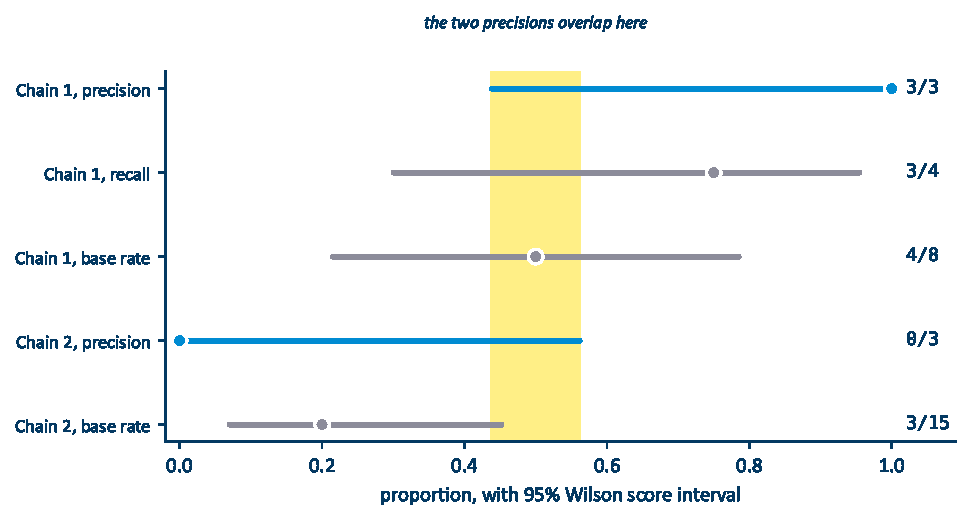
\includegraphics[width=0.94\linewidth]{Images/wilson_intervals.pdf}
    \caption[Interval estimates for the counted claims]{The five proportions with their Wilson
    intervals. The shaded band is the range the two precision intervals share: a precision of
    $1.00$ on three flags and one of $0.00$ on three flags are not, on this evidence,
    distinguishable.}
    \label{fig:wilson_intervals}
\end{figure}

The two precision rows are the ones that matter, and Figure~\ref{fig:wilson_intervals}
shows why: their intervals share the shaded band. The contrast between the two chains, which
Section~\ref{sec:res_second_chain} reads as a boundary, is therefore a difference between two point
estimates and not a demonstrated difference between two populations. That does not make the
boundary wrong, and the mechanism argued for it stands on its own; it means the boundary is
a hypothesis the campaign generated rather than a result the campaign established, and it is
reported as one.

\paragraph{What survives this, and why.}
Three findings do not depend on the size of the positive class, and they are the ones this
thesis rests on.

The first is structural. The defect located in Section~\ref{sec:res_mechanism} is a
property of a code path, not of a sample: the block in question cannot respond to the events
the scenario injects, which is verifiable by reading the propagation of a single event on a
single node and reproducible with one observation. A defect that is present in every run is
not made more or less true by how many runs there are.

The second is a theorem. The collapse of the criticality ranking under saturation is
Proposition~\ref{prop:saturation}, proved from the range and monotonicity of the propagation,
and the campaign merely provides an instance of it in nine turns of nineteen. No inference is
involved.

The third is a within-forecast comparison. The three outcome definitions of
Section~\ref{sec:res_target_trap} score the identical forecasts, so the spread between them
is a fact about the definitions and not an estimate of anything in a population. It needs no
interval because nothing is being generalised.

What does not survive is any statement of a rate. No number in this thesis should be read as
an estimate of how often the instrument would flag correctly in service, and the campaign was
never sized to produce one. Section~\ref{sec:future_work} gives the sample the question would
need.

\paragraph{The same standard applied to the one confirmed hypothesis.}
H5 is the single hypothesis this campaign confirms, and it is reported as a difference
between two means, $\Delta U_d = +0.079$ on press turns against $+0.005$ on calm turns at
nodes that are not physically affected. It carries no interval and no test, and applying the
protocol to the five negative verdicts while exempting the positive one would be the exact
asymmetry the protocol exists to prevent. The comparison is a paired one, the same nodes
observed under two conditions, so a permutation test on the turn labels is available and
costs nothing; it was not run because the per-node-turn declarations behind the two means are
not among the artefacts the derivation script of Section~\ref{sec:methods_repro} currently
exports. That is a reproducibility gap rather than a statistical one,  and it belongs on the list of
Section~\ref{sec:future_work}: until it is closed, H5 should be read as a
confirmed direction of effect and not as a measured effect size.

%% ═══════════════════════════════════════════════════════════════════════════
\subsection{Arm B: What Happens When the Forecast Is Shown}
\label{sec:res_armB}
%% ═══════════════════════════════════════════════════════════════════════════

Arm B replays the identical frozen scenario with the identical eight agents, changing one
thing: from turn 4 onward each agent is shown the predictive analysis of its own node before
declaring. The loop stays open, so the terrain does not change and the forecasts remain
scorable. One property of the design must be established before any interpretation: the
prediction layer is deterministic, so the two arms should carry identical forecasts on the
turns they share, and they do, all 72 shared node-turn forecasts being numerically identical.
Any behavioural difference therefore comes from the act of displaying the forecast, not from a
different forecast being displayed.

The dataset comprises 97 declaration records, reduced to 96 after removing one duplicate
submission at turn 1, each carrying an influence field recording whether the displayed
forecast had no influence, confirmed the agent's assessment, or caused an upward or downward
revision. Figure~\ref{fig:armB_influence} gives the distribution turn by turn.

The first exposure is the result. At turn 4, when the
forecast becomes visible for the first time, all eight agents record an influence and the
direction is entirely one-sided: five revised downward and three had their existing assessment
confirmed. Not one revised upward. The first upward revision anywhere appears at turn 5, and
the scenario's single critical event, the foundry accident, lands at turn 6, two turns after
the moment every declarant was either reassured or confirmed.

\begin{figure}[htbp]
    \centering
    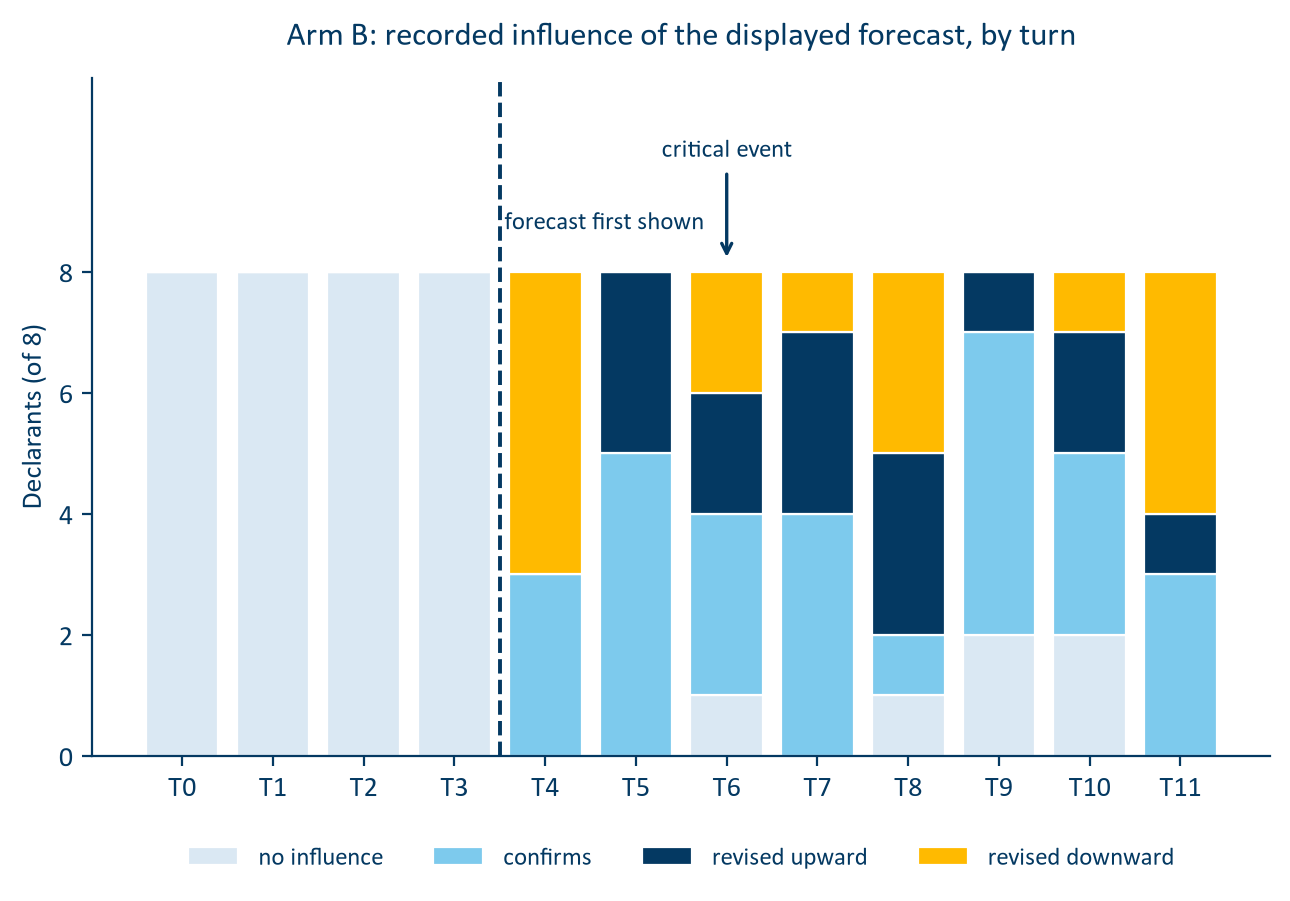
\includegraphics[width=0.86\linewidth]{Images/armB_influence.png}
    \caption{Arm B: influence of the displayed forecast, by turn}
    \label{fig:armB_influence}
\end{figure}

Over the full campaign the distribution is close to balanced, 15 upward against 16 downward,
so what the data shows is a strong first-exposure effect rather than a permanent suppression
of declared urgency. Two factors aggravate it. The forecast displayed at turn 4 is drawn from
the same layer whose confident predictions never materialise and whose $u_{\text{time}}$ block
is blind to the very shock about to arrive. And it is displayed as a numeric probability with
a confidence interval, a format the automation-bias literature identifies as increasing
reliance~\autocite{goddard2012automation,bansal2021whole}. The system was presenting an
unfounded reassurance in the most persuasive available form, immediately before the event it
had failed to anticipate.

One qualification cuts against the strongest reading. The influence field records the effect
on the declared urgency level, not on the decision taken, and the free-text notes show agents
continuing to negotiate allocation, alert the customer and order ahead of schedule at the same
turn. The measured effect is on what was declared rather than on what was done. Since the
declared value is precisely the input the adequacy layer consumes, that is still a
consequential effect on the measurement system.

\subsubsection{The Same Test on the Second Chain}
\label{sec:res_display_second_chain}

The airframer chain of Section~\ref{sec:res_second_chain} was then run a second time with the
forecast displayed, on the same indicator pack and the same derived truth as its control run,
so that the act of display is the only difference between the two. Fifteen declarants,
nineteen turns, 225 forecasts per arm, and 225 declarations made with a forecast on screen.
Figure~\ref{fig:benchmark_predict} carries the three measurements that follow.

Four results follow, and the first is a negative one that simplifies the method. The forecast
scores identically in both arms: a Brier skill of $-1.601$ against $-1.592$ at one week, an AUC
of $0.826$ in both, differences confined to the third decimal, and an unchanged node ranking.
The forecast is computed from indicators the declaration channel does not reach, so the loop is
too weak to close and a treatment arm can be scored exactly as a control arm can. The caution
stated when this campaign was designed, that showing the forecast would destroy the reference,
is refuted by measurement.

The second replicates first contact at five times the scale. On the turn the forecast first
appears, eleven of fifteen declarants report it confirms what they already thought, two revise
downward, and \emph{none} revises upward: the only turn in the campaign without a single upward
revision. One node states the mechanism in its own note, its second lot having sat at zero for
four consecutive turns, which should have raised its time-window urgency further, but the
tool's reading of eleven per cent tempered that concern. The forecast suppressed an escalation
the indicators warranted.

The third qualifies the first two and is the one that generalises. Across all fifteen turns
with a forecast visible, upward revisions outnumber downward ones $26$ to $9$: the one-sided
suppression is a first-exposure effect, and the persistent effect is different and larger. A
declarant follows the number in whichever direction it moves, one node raising its declared
urgency at turn~12 while its own indicators were improving because the tool had risen. The
display does not sedate the operator; it transfers authority from the shop floor to the model,
reassuring when the model is low and the ground is bad, alarming when the model is high and the
ground is good. On a layer whose Brier skill is $-1.59$ at one week, that transfer is the harm,
and it is the composition of two defects documented separately: miscalibration, and display.

The fourth was not sought, and it is the one a designer can act on. The share of declarants reporting that
the forecast changed nothing rises from two at turn~4 to twelve at turn~18, and over the last
four turns seventy-three per cent report no effect. Their reasons are measurable: between
consecutive turns, on the same node and with the terrain unchanged, the median move in the
four-week probability is $0.024$, but fourteen of $139$ moves exceed $0.20$, eight exceed
$0.50$, and the largest is $0.93$. A forecast that falls from thirty per cent to eight in one
turn teaches its reader to stop looking. Disengagement is a rational response to instability
rather than negligence, and it is more costly than the first-contact effect: by the closing
turns, when the layer finally does place a high probability on the supplier that goes on to
miss, no one is reading it.

\begin{figure}[htbp]
\centering
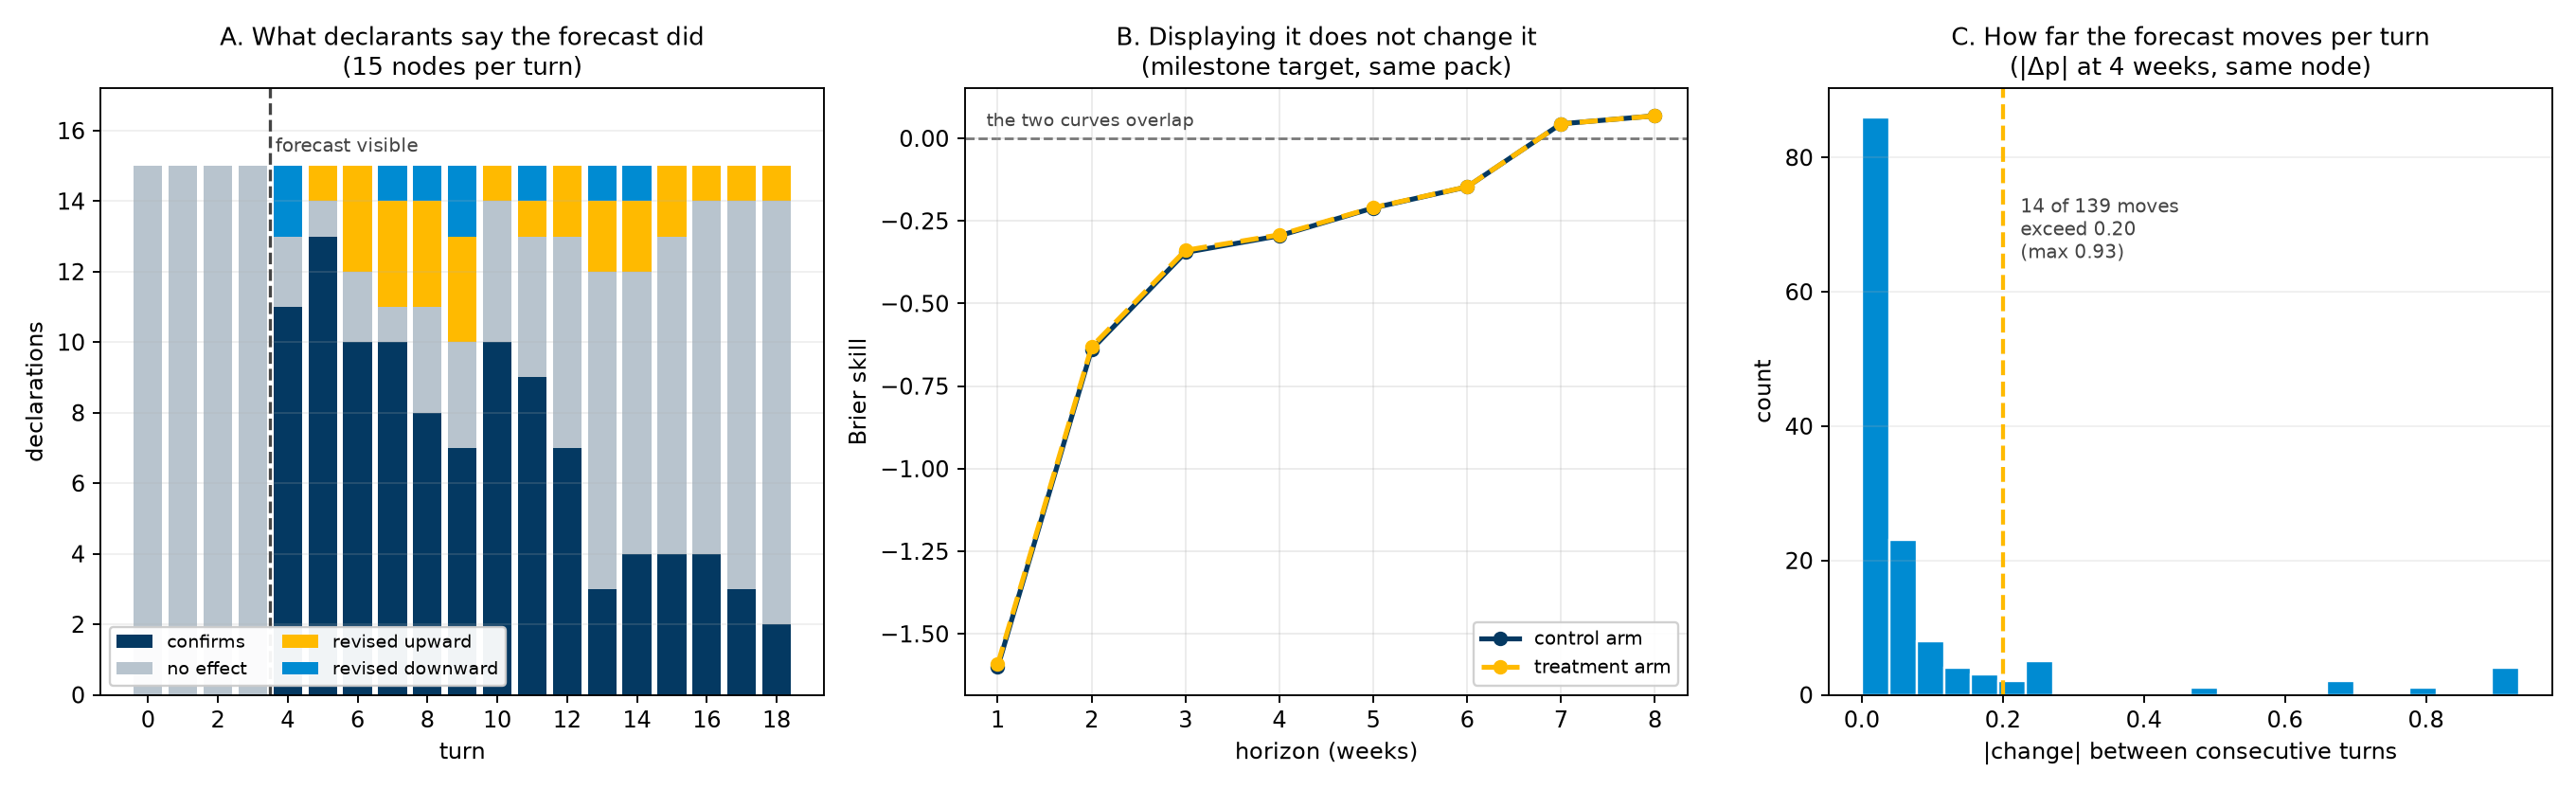
\includegraphics[width=\linewidth]{Images/benchmark_predict.png}
\caption[Displaying the forecast: what changes and what does not]{The second chain, run twice
on one indicator pack. \textbf{A}: what declarants report the forecast did to their judgement,
by turn: first contact at turn~4 produces no upward revision at all, and reported influence
decays as the campaign proceeds. \textbf{B}: the forecast scores identically whether or not it
is displayed; the two curves overlap. \textbf{C}: the turn-to-turn movement of the four-week
probability on an unchanged node, which is what declarants cite when they stop trusting it.}
\label{fig:benchmark_predict}
\end{figure}

\subsubsection{What the Model Being Followed Actually Knows}
\label{sec:res_trivial_baseline}

The preceding result rests on a premise worth testing: that the layer declarants defer to is
doing work a declarant could not do unaided. Two observations put that in doubt. Enriching two
dead indicator blocks on this chain moved computed urgency on $174$ of $285$ node-turns and
left the forecast identical to nine decimal places on $151$ of $154$ comparable points, and
reading the simulation loop explains why. The autoregressive state fitted to local urgency
enters only the client-impact channel; the scored outcome is the disjunction of a milestone
term and an event term, the milestone term depends only on a lead-time draw against the
fraction of the milestone still outstanding, and the event term is empty on a chain carrying no
exogenous shock. Computed urgency never reaches the quantity being scored.

That is a claim about code, so it was tested against a baseline built to be as weak as
possible. For a node whose next unfinished milestone falls due at turn $D$ with fraction $r$ of
its work outstanding and nominal lead time $L$ in turns, the baseline announces
$p(k) = \mathrm{clip}(1 - (D - t - k)/rL,\,0,\,1)$: no simulation, no fitted parameter, no
calibration and none of the six urgency blocks. The service declines to forecast on $71$ of the
$225$ node-turns, where no milestone is in flight, and the baseline is silenced on exactly
those, so both are scored on an identical sample at every horizon.

\begin{figure}[htbp]
\centering
\begin{tikzpicture}[x=1cm, y=1cm, font=\scriptsize,
    bx/.style = {bloc, text width=4.4cm, minimum height=1.15cm, align=left, inner xsep=5pt}]

\node[bx, blocFort] (sim) at (3.0, 1.5)
     {\textbf{the forecast layer}\\500 Monte Carlo trajectories,\\AR(1), Beta posterior,
      bootstrap};
\node[bx, blocAlerte] (base) at (3.0, -0.6)
     {\textbf{the baseline}\\one line: work outstanding\\divided by nominal lead time};

\node[bx, text width=3.6cm] (auc) at (9.2, 1.5)
     {AUC at 1w and 2w\\$0.583$ and $0.544$};
\node[bx, text width=3.6cm] (aucb) at (9.2, -0.6)
     {AUC at 1w and 2w\\$\mathbf{0.667}$ and $\mathbf{0.633}$};

\node[bx, text width=3.2cm, blocPale] (bs) at (13.2, 1.5)
     {Brier skill $-1.601$};
\node[bx, text width=3.2cm, blocPale] (bsb) at (13.2, -0.6)
     {Brier skill $-4.851$};

\draw[fleche] (sim) -- (auc);
\draw[fleche] (base) -- (aucb);
\draw[fleche] (auc) -- (bs);
\draw[fleche] (aucb) -- (bsb);

\node[etiquette, anchor=north, text width=11.5cm] at (7.0, -1.35)
     {the baseline orders better at six horizons of eight and cannot state a level at all:
      ordering and calibration are separate properties, and the expensive machinery bought
      only the second};

\end{tikzpicture}
\caption[A one-line baseline against the simulation]{The comparison that decides whether the
forecast layer earns its complexity. The baseline is silenced on the 225 node-turns where no
milestone is in flight, and on the rest it ranks the misses better while producing no usable
probability.}
\label{fig:baseline}
\end{figure}

The baseline ranks the misses \emph{better} than five hundred Monte-Carlo trajectories at six
horizons of eight. At one week its AUC is $0.908$ against $0.826$ and its PR-AUC $0.396$
against $0.153$; the Monte-Carlo layer regains the advantage only at seven and eight weeks
($0.667$ and $0.633$ against $0.583$ and $0.544$). Since the baseline reads the remaining
fraction from the same progress variable the truth is derived from, it was re-run in a form
that reads nothing at all, remaining work taken as the calendar fraction a perfectly healthy
milestone would show, using only the due date and the nominal lead time. Its AUC and PR-AUC are
identical to three decimal places at every horizon. The discrimination is entirely the ratio of
weeks remaining to weeks required.

What the simulation layer does contribute is visible in the same table and is not
discrimination. Its Brier skill is $-1.601$ at one week against the baseline's $-4.851$: the
baseline produces an ordering and has no means of turning it into a probability, and converting
an ordering into a scale is what the five hundred trajectories are doing. It also holds its
ranking at the long horizons where a calendar ratio collapses, at nearly double the PR-AUC at
seven and eight weeks. The layer is therefore a calibration wrapper around a lead-time ratio,
which is a defensible thing to be, but it is not what the interface presents and not what the
declarants in Section~\ref{sec:res_display_second_chain} believed they were deferring to.

This sharpens rather than softens the display result. Twenty-six upward revisions and nine
downward ones were made in deference to a short-horizon signal that a two-number ratio
reproduces and slightly exceeds: the transfer of authority documented above was not a transfer
to a model that knew more but, at the horizons displayed, to one that knew less. The defect is
nameable and cheap to repair, since the autoregressive state must enter the milestone term and
not only the client-impact term, and the repair would be measurable on these same frozen
forecasts. It was not attempted here, and the sample bounds it: five positives at one week, one
chain, one outcome definition.

%% ═══════════════════════════════════════════════════════════════════════════
\subsection{The Repair, in Brief}
\label{sec:res_repair}

The defect of Section~\ref{sec:res_mechanism} was repaired and the identical frozen forecasts
were rescored against it. Two results belong in the body and the working is in
Appendix~\ref{app:repair}.

The repair changed the recommendation as well as the model. Routing the calibrated events into
the lead time, which is the obvious reading of the diagnosis, does not work: a quantity routed
that way is scaled by the fraction of work remaining, so it attenuates to nothing on exactly
the milestones nearest their deadline. Lost time has to be added to the completion date
instead. The diagnosis was right and the instruction it implied was wrong, which was only
visible because the repair was re-measured rather than assumed to work.

What it bought is bounded. The structural repair lifts both calibration and discrimination at
every horizon, the Brier deficit roughly halving from $-0.553$ to $-0.216$ at four weeks. The
system moves from badly wrong to less wrong, not to useful, and the Brier skill remains
negative throughout. Two further defects surfaced with it: the forecast treated declared
progress as exact, which made the milestone probability binary in $85\%$ of cases, and the
campaign ran at $25.6\%$ indicator coverage with three of six blocks inert.

\subsection{Discussion}
\label{sec:res_discussion}
%% ═══════════════════════════════════════════════════════════════════════════

Six threads run through this discussion and they are not claims of the same kind. Four
survive the sample size because they concern how a measurement is built; two do not,
because they concern how often something happened. Reading them as though they were
equivalent is how a campaign of this size gets over-read.

\paragraph{The circularity problem is the central methodological finding.}
Across the dry run, arm A and arm B, the same difficulty recurs in three different forms.
In the dry run, synthetic declared urgency was anchored on real urgency by construction, so
the gap the system exists to measure could not appear. In arm A, agents read their briefings
carefully and declared close to what the briefing described, so the gap again did not
appear, with $H$ peaking at $0.017$ where the hypothesis required $0.3$. In arm B, showing
the model's own output to the declarant closed the loop explicitly, so the declaration is
no longer independent of the model at all. A system that measures the divergence between a
human judgement and a computed state is only measuring anything when those two quantities
have independent sources. I expected that to be a property of the design. It turned out to
be a property that has to be defended in three separate places, and I missed it in all
three before the data showed me.

\paragraph{Ordering and level are separate problems needing separate fixes.}
The scores of Section~\ref{sec:res_armA_scored} do not support a single verdict on the
forecast layer. On this campaign it neither orders well nor announces well, but the
evidence for those two claims is of very different strength: discrimination rests on between
two and six positive observations and is therefore inconclusive, while the calibration
failure rests on 21 confident forecasts none of which materialised and is not plausibly a
sampling artefact. The remedies differ accordingly. Miscalibration of this shape is
routinely corrected by a post-hoc layer without touching the underlying
model~\autocite{niculescu2005predicting,guo2017calibration}. Poor discrimination is not, and
would require the model to change.

\paragraph{The specific defect is repairable and general, but not in the obvious way.}
The mechanism identified in Section~\ref{sec:res_mechanism} is not a scenario artefact. The
$u_{\text{time}}$ block computes milestone risk from a lead-time distribution against a
deadline, while the event engine writes to capacity, cost and failure probability. No path
connects a shock to any quantity on the time axis, so the block cannot respond to a
disruption, and any deployment of this framework would inherit that gap. The natural repair is to make the calibrated events write a lead-time impact, and
Section~\ref{sec:res_repair} reports that this was implemented, measured and found to be
wrong. The general form of the lesson is that a parameter describing a node's capacity to
recover and a state accumulating what it has already lost carry the same units and are easy to
confuse, and the confusion stays invisible while the database is incomplete.

\paragraph{Communicating ignorance is a design requirement, not a nicety.}
The arm B result reframes what an advisory layer owes its reader. Faced with an exogenous
shock, a weather event, a fire, a geopolitical decision, the model has no basis for
prediction at all. Displaying a low probability in a confident format is then worse than
displaying nothing, because it converts an absence of information into an apparent
reassurance. Two mitigations follow and neither requires new science: make the
horizon salient, so that a low four-week probability cannot be read as a general statement of
safety, and state explicitly which classes of risk the model does not cover. I would now treat
both as acceptance criteria for an advisory layer rather than as refinements to add later.

\paragraph{Threats to validity.}
Four limit what the above can support. The declarants are language models, so the external
validity of any claim about human declaration behaviour is unestablished; this is the
principal threat, and it is why arm B is reported as a measured effect on this population
rather than as a finding about operators. The campaign is a single scenario, so the outcome
base rate, the event mix and the milestone structure are all properties of one script. The
positive class is very small, which bounds every discrimination claim. Finally, arm B is
not blinded, since the agents are told they are being shown a predictive analysis; a design
in which some turns show a deliberately uninformative forecast would separate the effect of
the content from the effect of the display.

\paragraph{Against the pre-registered thresholds.}
Five of the six hypotheses are not confirmed and one, H5 on urgency contagion, is confirmed.
That is a largely negative result against the register, and it is reported as such. The
value of the campaign lies less in those verdicts than in the diagnosis they made possible:
the register asked whether the signal works, and the answer, with its mechanism, is that one
identifiable block prevents it from working and that showing the resulting forecast to the
declarant is actively counterproductive until that block is fixed.

%% ═══════════════════════════════════════════════════════════════════════════
